\documentclass[11pt,a4paper]{article}

\usepackage[margin=1in]{geometry}
\usepackage[T1]{fontenc}
\usepackage[utf8]{inputenc}
\usepackage{lmodern}
\usepackage{microtype}
\usepackage{amsmath,amssymb,amsfonts,amsthm}
\usepackage{mathtools}
\usepackage{graphicx}
\usepackage{booktabs}
\usepackage{array}
\usepackage{enumitem}
\usepackage{xcolor}
\usepackage{float}
\usepackage{caption}
\usepackage{hyperref}
\usepackage{authblk}
\usepackage{tikz}
\usetikzlibrary{arrows.meta,positioning,fit}

\usepackage[
    backend=biber,
    style=authoryear,
    sorting=nyt,
    maxcitenames=2,
    maxbibnames=99,
    giveninits=false,
    uniquename=false,
    uniquelist=false,
    doi=true,
    url=true,
    isbn=false,
    eprint=true
]{biblatex}

\addbibresource{references.bib}
\DeclareDelimFormat{nameyeardelim}{\addspace}
\setlength{\bibhang}{1.5em}
\DeclareFieldFormat[article,inproceedings,incollection]{title}{\mkbibquote{#1}}
\DeclareFieldFormat[book,report,thesis,misc]{title}{\mkbibemph{#1}}
\DefineBibliographyStrings{english}{
  andothers = {et\addabbrvspace al\adddot}
}

\newtheorem{proposition}{Proposition}
\newtheorem{corollary}{Corollary}
\newtheorem{definition}{Definition}
\newtheorem{remark}{Remark}
\newtheorem{assumption}{Assumption}

\newcommand{\X}{\ensuremath{\mathcal{X}}}
\newcommand{\Z}{\ensuremath{\mathcal{Z}}}
\newcommand{\ThetaSpace}{\ensuremath{\Theta}}
\newcommand{\EtaSpace}{\ensuremath{\mathcal{E}}}
\newcommand{\Mnominal}{\ensuremath{\mathcal{M}_{\mathrm{N}}}}
\newcommand{\Gnuis}{\ensuremath{G_{\mathrm{nuis}}}}
\newcommand{\R}{\ensuremath{\mathbb{R}}}
\newcommand{\quotient}{\ensuremath{\mathcal{X}/G_{\mathrm{nuis}}}}
\newcommand{\taumc}{\ensuremath{\tau_{\mathrm{MC}}}}
\newcommand{\taustar}{\ensuremath{\tau_k^\star}}

\title{
\large
\textbf{Fleet-Wide Condition Monitoring via Shared Nominal Representations and Local Radius Calibration}\\
\medskip
Enabling OEM-Centralized, Fleet-Deployed CBM
}

\author[1]{Eduardo Di Santi}
\affil[1]{Department of Applied Mathematics, University of Colorado Boulder
}
\date{}

\begin{document}
\maketitle

%=====================================================================
% Abstract
%=====================================================================
\begin{abstract}

\textbf{Objectives:} Transportation operators deploying condition monitoring
across large fleets of heterogeneous assets rarely have fault labels, time
for per-asset representation learning, or long field calibration campaigns.
This paper addresses how a single nominal representation can be deployed
fleet-wide on day one, without retraining a model or tuning a threshold for
every asset.

\textbf{Methods:} A canonical nominal representation, a Conv1D autoencoder,
is trained once offline on simulated healthy signals and
transferred unchanged to every asset. Each asset then estimates its
operational radius, an empirical residual quantile, from a short stream of
unlabeled local observations, without retraining the shared model. The
method is evaluated on four Case Western Reserve University (CWRU) bearing
conditions, spanning healthy, ball-fault, inner-race, and outer-race
windows, against an oracle calibrated on each condition's complete healthy
dataset. Three calibration strategies are compared: direct threshold
transfer, a complete-data oracle radius, and the proposed online radius
estimated from only the first 100 healthy windows.
The deployment principle is further validated on four independently
monitored bearings from the NASA IMS run-to-failure dataset and compared
with autoencoders trained separately on each bearing's early-life data.


\textbf{Findings:} Direct transfer of the absolute simulator threshold
produced complete false alarms in the field, confirming that the
representation, not its absolute score scale, transfers. Using only a
100-window online calibration, the shared representation reached an
average healthy false-alarm rate of 3.09\%, ball-fault detection of
99.69\%, and 100\% detection of inner- and outer-race faults, with the
radius converging after 51.0 $\pm$ 12.6 windows, approaching the
asset-specific reference.
On NASA IMS, the shared representation detected persistent departure in
all four bearings, on average 83.25 hours before the documented end of the
experiment, compared with 47.89 hours for the per-asset early-life
autoencoders, while eliminating per-asset representation training.

\textbf{Novelty:} The contribution is a fleet-deployment methodology, not a
new anomaly-detection architecture: it separates representation learning,
performed once and shared fleet-wide, from decision-boundary calibration,
performed independently by each asset.

\textbf{Practical Applications:} A shared representation can be developed
and maintained centrally, for example by an original equipment
manufacturer, and distributed unchanged across an operator's fleet, while
each installed asset requires only seconds of unsupervised local
calibration and lightweight edge inference, removing the need for fault
labels or per-asset model training during rollout.

\end{abstract}

\vspace{0.3cm}
\noindent\textbf{Keywords:}
fleet-wide condition monitoring,
shared nominal representation,
simulation-to-field model transfer,
local threshold calibration,
run-to-failure monitoring,
condition-based maintenance

%=====================================================================
\section{Introduction}
\label{sec:introduction}
%=====================================================================

Modern transportation systems increasingly rely on condition-monitoring technologies to supervise
large populations of operational assets, including rolling-element bearings, axleboxes, traction
motors, gearboxes, pumps, actuators, vehicles, and spatially indexed infrastructure segments
\cite{jardine2006,zhao2019}. Although machine-learning research has produced increasingly capable
anomaly detectors \cite{chandola2009,zhao2019}, the deployment problem remains largely unresolved:
a detector that performs well for one asset under one calibrated operating condition does not
automatically scale to hundreds or thousands of independently installed units.

At fleet rollout, several constraints arise simultaneously. First, the target fleet contains few
or no representative fault examples. Second, waiting months or years for failures to accumulate
is operationally unacceptable. Third, installation-specific factors such as sensor coupling,
mounting, operating point, and environmental noise alter the numerical scale of anomaly scores
between assets \cite{randall2011}. Fourth, training, calibrating, validating, and maintaining a
separate representation model for every physical unit creates an operational and organizational
burden that grows directly with fleet size.

The practical question is therefore not simply

\begin{quote}
\emph{How can an anomalous condition be detected?}
\end{quote}

but rather

\begin{quote}
\emph{How can one nominal representation be deployed on day one across a heterogeneous fleet
while retaining performance close to an ideal asset-specific solution, without per-asset
representation learning or manual threshold tuning?}
\end{quote}

This paper addresses that question by separating representation engineering from deployment
calibration. A canonical nominal representation is learned once, offline, from simulated healthy
observations and is distributed unchanged across the fleet. Each deployed asset estimates only
its own operational radius from a short stream of unlabeled local observations. The shared model
is not retrained, fine-tuned, or adapted in the field.

From a broader perspective, this separation can be interpreted as an inverse problem.
Representation learning is performed once to recover a canonical nominal representation from
observations, whereas deployment requires each asset to solve only a lightweight local inverse
calibration problem by identifying its own operational radius around that fixed representation.
This interpretation follows the inverse-problem and quotient-space formulations introduced in our
previous work \cite{disanti2026inverse,disanti2026quotient}, while the present paper focuses on
their engineering realization for scalable fleet deployment.

For asset $k$, let $\tau_k(t)$ denote the progressively estimated operational radius. Under stable
nominal operation, the proposed calibration procedure is expected to satisfy

\[
\tau_k(t)\rightarrow\tau_k^\star,
\]

where $\tau_k^\star$ is an asset-specific acceptance boundary around the fixed shared
representation. Once convergence is established, the radius is frozen or tightly constrained so
that subsequent degradation cannot redefine itself as nominal through unrestricted adaptation.

The distinction between the transferable representation and the local decision boundary is
essential. A reconstruction-error threshold learned in simulation is expressed in the numerical
scale induced by the simulator, its preprocessing, and its residual distribution. Applying that
absolute value directly to a field installation may therefore fail even when the underlying
representation remains diagnostically useful. The proposed method transfers neither an absolute
threshold nor an asset-specific model. Instead, it transfers the canonical nominal representation
and a fleet-wide target nominal coverage, while each asset estimates the empirical residual
quantile that realizes that coverage locally.

The transferable object is therefore not an anomaly threshold, but a canonical nominal
representation. Deployment consists only of identifying the local operational radius around that
shared representation.

This formulation also changes the relevant experimental comparison. The ideal reference is not
another globally shared detector, but an operationally unrealistic condition in which the
complete healthy distribution of every asset is available in advance and a separate detector can
be trained and calibrated for each one. The central question is therefore

\begin{quote}
\emph{How much detection performance is lost when many asset-specific models are replaced by one
simulator-trained representation and a few seconds of local calibration?}
\end{quote}

We first answer this question under controlled operating-condition
heterogeneity using four CWRU \cite{smith2015} conditions, and then evaluate its extension
to independently monitored physical units and naturally evolving
degradation using the NASA IMS run-to-failure dataset.

The asset-specific reference methods are trained and calibrated using the complete healthy dataset of each condition. In contrast, the proposed method
uses no field observation for representation learning and estimates its local operational radius
from only the first 100 healthy windows, corresponding to approximately ten seconds of signal at
the evaluated window duration.

The experimental results show that the cost of scalable deployment is small. Asset-specific
autoencoders reach 100\% detection across the evaluated ball-, inner-race-, and outer-race-fault
families. The unchanged simulator-trained shared model, combined with online local-radius
estimation, reaches an average ball-fault detection rate of 99.69\% and 100\% detection of
inner- and outer-race faults. The operational radius converges after
$51.0\pm12.6$ windows on average. Direct transfer of the absolute simulator threshold, however,
produces 100\% healthy false alarms, confirming that the representation transfers while its
absolute score scale does not.

The contribution of this paper is therefore a deployment methodology rather than a new neural
architecture. Although a Conv1D autoencoder is used as the experimental representation, the
deployment principle is representation-agnostic. The principal contributions are:

\begin{enumerate}[leftmargin=1.5em]
    \item a fleet-wide architecture that separates one shared canonical nominal representation
    from independently calibrated local operational radii;

    \item a direct simulation-to-field experiment in which the representation is transferred
    unchanged and no field data are used for representation learning;

    \item an online empirical-quantile calibration procedure that estimates an asset-specific
    operational radius from a short unlabeled warm-up;

    \item a convergence criterion that separates finite cold-start calibration from subsequent
    degradation monitoring;

    \item a comparison against ideal asset-specific detectors trained and calibrated with the
    complete healthy dataset of every evaluated condition; and

    \item an edge-oriented deployment model in which the representation may be produced and
    maintained centrally---for example by an original equipment manufacturer---while each
    deployed unit performs only lightweight local calibration.
\end{enumerate}

The methodology is intentionally independent of asset type and sensing modality. It requires only
a nominal representation producing a scalar anomaly score, repeated observations from each
operational unit, and a local procedure for estimating the acceptance boundary. Public
rolling-element bearing data are used here as the first controlled validation domain rather than
as a limitation of the proposed methodology.

The remainder of the paper is organized as follows. Section~\ref{sec:related} reviews condition
monitoring, one-class anomaly detection, adaptive calibration, and fleet deployment.
Section~\ref{sec:method} defines the shared representation and local operational-radius
estimation. Section~\ref{sec:expdesign} presents the experimental protocol.
Section~\ref{sec:results} reports the deployment-oriented results, and
Section~\ref{sec:discussion} discusses industrial implications, limitations, and future work.
Section~\ref{sec:theory} summarizes the underlying mathematical interpretation.

%=====================================================================
\section{Related Work}
\label{sec:related}
%=====================================================================

Condition-based maintenance (CBM) has become a central component of modern transportation asset
management, with condition monitoring providing the operational evidence required to supervise
large fleets of heterogeneous assets
\cite{jardine2006,chandola2009,zhao2019}. Although the sensing modality depends on the
application---including vibration, acoustic emission, electrical current, temperature, strain,
or other physical measurements---the computational objective is fundamentally the same: to
characterize nominal operation and detect persistent departures that may indicate degradation.

Most machine-learning approaches formulate this problem as supervised fault classification,
assuming representative fault examples are available during training. While effective on
benchmark datasets, supervised methods require fault labels and generally assume that deployment
conditions remain close to those observed during model development.

One-class and novelty-detection methods, including one-class SVM
\cite{scholkopf1999}, neural-network novelty detection \cite{bishop1994}, and
autoencoder-based anomaly detection \cite{hinton2006,sakurada2014}, reduce the dependence on
fault labels by learning only nominal behaviour. More recently, representation-learning
approaches have substantially improved anomaly detection by constructing latent spaces in which
healthy operation occupies a compact region while degraded behaviour becomes more easily
separable.

However, the overwhelming majority of existing work focuses on learning better anomaly
detectors. Comparatively little attention has been paid to the deployment problem itself:
how a single nominal representation should be initialized, calibrated, and maintained across a
heterogeneous fleet of independently operating assets.

Adaptive thresholds are frequently employed in streaming anomaly detection to compensate for
changes in operating conditions. However, unrestricted adaptation introduces an important
operational risk: persistent degradation may progressively redefine itself as nominal by
continuously shifting the decision boundary. This observation motivates separating calibration
from monitoring. In the proposed methodology, adaptation is restricted to a finite cold-start
phase whose objective is to estimate an operational radius for each asset. Once convergence has
been achieved, the shared representation remains fixed and subsequent departures become
diagnostic evidence rather than input for further adaptation.

The present work is also related to invariant representation learning
\cite{bronstein2021} and anomaly detection under distribution shift
\cite{li2023invariant}, which seek representations that are insensitive to operationally
irrelevant variability. Our contribution, however, lies at a different level of the
condition-monitoring pipeline. Rather than proposing a new representation-learning architecture,
we address the deployment problem itself: how a shared nominal representation can be deployed
across heterogeneous assets through shared nominal coverage, independent operational-radius
convergence, and local empirical calibration, without fault labels or per-asset retraining.

From a broader perspective, this deployment strategy follows the viewpoint that diagnosis should
recover a canonical nominal representation from observations, while deployment should estimate
only the local neighbourhood in which that representation remains valid for each individual
asset. This interpretation is consistent with the inverse-problem and quotient-space
formulations introduced in our previous work
\cite{disanti2026inverse,disanti2026quotient}, although the present paper focuses exclusively on
the engineering problem of scalable fleet deployment.

The methodology is intentionally independent of both sensing modality and asset type. The
present manuscript validates the approach on the CWRU bearing benchmark
\cite{smith2015} because it provides controlled nominal observations, multiple fault modes,
and several operating conditions. Bearings should therefore be interpreted as the first
validation domain rather than as a limitation of the proposed deployment method.

Accordingly, this paper should be interpreted not as proposing another anomaly-detection
architecture, but as introducing a deployment methodology in which a shared canonical nominal
representation is combined with independent operational-radius convergence for each monitored
asset.

%=====================================================================
\section{Method}
\label{sec:method}
%=====================================================================

The objective of the proposed methodology is not to learn a detector for each
asset independently, but to separate two distinct problems: learning a single
shared canonical nominal representation for the fleet and estimating an
asset-specific operational radius during deployment.

This section formalizes that deployment architecture.

\subsection{Deployment architecture: shared representation, local radius}

Let $x_{k,t}\in\X$ denote an observation window acquired from operational unit $k$ at time
$t$. In the bearing validation presented in this paper, $x_{k,t}$ is instantiated as a
fixed-length vibration window. A shared
offline-trained representation model produces an anomaly score
\begin{equation}
r_{k,t}=r(x_{k,t}).
\label{eq:score}
\end{equation}

The representation model is common to the fleet. The decision boundary is not. Each asset
maintains a local operational radius $\tau_k(t)$ and raises an alarm when
\begin{equation}
r_{k,t}>\tau_k(t).
\label{eq:decision}
\end{equation}

The method therefore enforces three deployment rules:

\begin{enumerate}[leftmargin=1.5em]
    \item the representation is shared;
    \item the calibration is local;
    \item the model is never retrained per asset.
\end{enumerate}

\begin{figure}[H]
\centering
\fbox{
\begin{minipage}{0.88\linewidth}
\centering
\textbf{Shared offline nominal model}\\[0.15cm]
$\downarrow$\\[0.1cm]
\begin{tabular}{ccc}
Asset A & Asset B & Asset C\\
$\tau_A(t)\rightarrow\tau_A^\star$ &
$\tau_B(t)\rightarrow\tau_B^\star$ &
$\tau_C(t)\rightarrow\tau_C^\star$
\end{tabular}\\[0.2cm]
\textit{Shared representation; independent operational-radius convergence.}
\end{minipage}}
\caption{Fleet deployment architecture. One representation is distributed fleet-wide, while
each physical asset converges independently to its own operational radius.}
\label{fig:deployment-architecture}
\end{figure}

\begin{definition}[Operational radius]
For a fixed nominal representation and an independently monitored operational unit $k$, the
operational radius $\tau_k^\star$ is the converged, asset-specific acceptance boundary estimated
from nominal deployment observations. It calibrates the anomaly decision locally without
modifying or retraining the shared representation.
\end{definition}

\subsection{Representation instantiation}

The deployment method is independent of the representation backbone. In this paper, we
instantiate it with a Conv1D autoencoder $A_\phi=D_\phi\circ E_\phi$ trained exclusively on
nominal signals. The encoder maps a 1200-sample window through three Conv1D layers
(32, 64, and 128 filters) to a 16-dimensional latent code with an $\ell_1$ activity penalty; the
decoder mirrors this structure with Conv1DTranspose layers. The model has 847,601 parameters
and is trained with Adam, mean-squared reconstruction loss, early stopping, and learning-rate
decay.

The anomaly score is the reconstruction residual
\begin{equation}
r(x)=\|x-A_\phi(x)\|_2^2.
\label{eq:residual}
\end{equation}

The autoencoder is merely one possible instantiation of the shared representation. The scientific contribution is the deployment methodology rather than the particular representation-learning architecture.
Any nominal representation producing a stable scalar distance or anomaly score could replace
Equation~\ref{eq:residual}.

\begin{figure}[H]
\centering
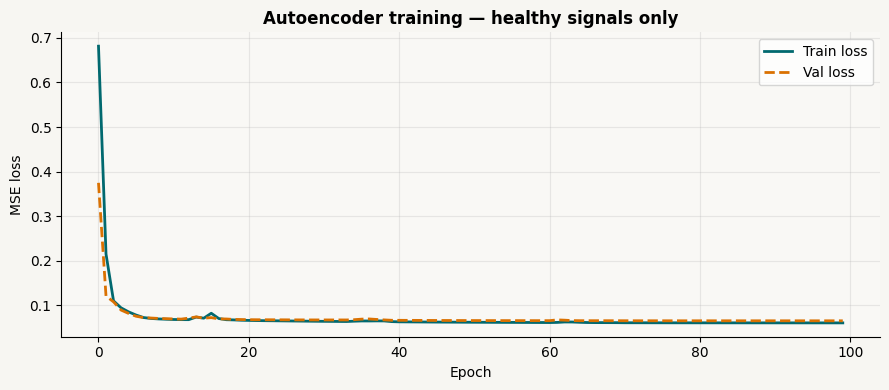
\includegraphics[width=0.78\linewidth]{training.png}
\caption{Training and validation loss of the healthy-only Conv1D autoencoder used as the shared
nominal representation.}
\label{fig:ae-training}
\end{figure}

\subsection{Shared nominal coverage and local empirical radius}

The fleet-wide calibration parameter is a target nominal coverage level
$1-\alpha$, rather than an absolute anomaly-score threshold. In the present
experiments, $1-\alpha=0.98$.

For operational asset $k$, let
$\widehat{Q}_{k,t}(1-\alpha)$ denote the empirical $(1-\alpha)$-quantile of
the local residuals observed during initialization up to time $t$. The local
operational radius is

\begin{equation}
\tau_k(t)=\widehat{Q}_{k,t}(1-\alpha).
\label{eq:adaptive}
\end{equation}

The simulator threshold

\begin{equation}
\tau_{\mathrm{MC}}
=
\widehat{Q}_{\mathrm{MC}}(1-\alpha)
\end{equation}

is retained only for comparison. Its absolute numerical value is
not used by the proposed field-deployment procedure. What is shared across
the fleet is the target nominal coverage, while each asset identifies the
residual value that realizes that coverage locally.
\begin{figure}[H]
\centering

\begin{tikzpicture}[
    >=Latex,
    node distance=1.8cm,
    every node/.style={font=\small}
]

% Shared representation
\node[draw,rounded corners,minimum width=3.5cm,minimum height=1.0cm] (ae)
{Shared nominal representation};

% Residuals
\node[draw,rounded corners,below left=1.6cm and 2.2cm of ae,
minimum width=3.2cm] (a)
{Asset A residuals};

\node[draw,rounded corners,below=1.6cm of ae,
minimum width=3.2cm] (b)
{Asset B residuals};

\node[draw,rounded corners,below right=1.6cm and 2.2cm of ae,
minimum width=3.2cm] (c)
{Asset C residuals};

% arrows
\draw[->] (ae) -- (a);
\draw[->] (ae) -- (b);
\draw[->] (ae) -- (c);

% local radius

\node[below=0.8cm of a] {$\tau_A^\star$};

\node[below=0.8cm of b] {$\tau_B^\star$};

\node[below=0.8cm of c] {$\tau_C^\star$};

\draw[->] (a) -- ++(0,-0.45);
\draw[->] (b) -- ++(0,-0.45);
\draw[->] (c) -- ++(0,-0.45);

\end{tikzpicture}

\caption{
The same shared nominal representation produces reconstruction residuals for every deployed asset.
Only the local empirical residual distribution changes across installations.
Each asset independently estimates its own operational radius
$\tau_k^\star$, while the representation remains unchanged.
}
\label{fig:shared_local}
\end{figure}


\subsection{Operational-radius convergence}

During cold start, each asset collects a short sequence of initialization residuals and updates
Equation~\ref{eq:adaptive}. The asset is considered calibrated when the radius stabilizes.

For a look-back interval $L$, define the convergence statistic
\begin{equation}
C_k(t)=
\frac{\left|\tau_k(t)-\tau_k(t-L)\right|}
{\max\left(\tau_k(t-L),\epsilon\right)},
\label{eq:convergence}
\end{equation}
where $\epsilon>0$ prevents division by zero.

Calibration is declared when
\begin{equation}
C_k(t)<\varepsilon_C
\end{equation}
for $m$ consecutive updates. The converged operational radius is then
\begin{equation}
\tau_k^\star=\tau_k(t_{\mathrm{conv}}).
\label{eq:taustar}
\end{equation}

The key hypothesis evaluated in this paper is:

\begin{quote}
\emph{Under stable nominal operation, every asset converges rapidly to its own operational
radius around a fixed shared representation.}
\end{quote}

After convergence, $\tau_k^\star$ is frozen or allowed only a tightly bounded robust correction.
This prevents a slowly increasing anomaly score from being absorbed as a new nominal state.

The convergence criterion therefore defines the transition from representation
calibration to operational monitoring.

\subsection{Guarded updates}

For deployment beyond the controlled warm-up evaluated here, a guarded update rule can be applied to the local baseline. Let $\delta>0$ define a
guard band. A residual updates the local statistics only when
\begin{equation}
r_{k,t}<\tau_k(t)-\delta.
\label{eq:safe-update}
\end{equation}

Samples inside the guard band are observed but do not update the baseline, and samples above
$\tau_k(t)$ are flagged as anomalous. The three regions are therefore:

\begin{align}
r_{k,t}<\tau_k(t)-\delta
&\quad\Rightarrow\quad \text{safe update},\\
\tau_k(t)-\delta\le r_{k,t}\le\tau_k(t)
&\quad\Rightarrow\quad \text{observe, do not update},\\
r_{k,t}>\tau_k(t)
&\quad\Rightarrow\quad \text{anomaly}.
\end{align}

This rule is deliberately lightweight: each asset stores only a residual buffer or running robust
statistics, its current radius, and its convergence state.

\subsection{Deployment states}

Each asset transitions through three operational states:

\begin{enumerate}[leftmargin=1.5em]
    \item \textbf{Cold start:} the target nominal coverage is converted into a local empirical
operational radius from the incoming residual stream;
    \item \textbf{Converged nominal:} $\tau_k^\star$ has stabilized and monitoring is active;
    \item \textbf{Departure:} persistent scores exceed the converged radius.
\end{enumerate}

A practical alarm may require $q$ exceedances within the last $p$ observations to avoid reacting
to isolated impulses.

%% ------------------------------------------------------------------
%% Scope of the method (recommended addition)
%% ------------------------------------------------------------------
\subsection{Scope of the Method}

The deployment mechanism proposed in this paper is intentionally asset-agnostic.
Throughout the paper, the index $k$ denotes an independently monitored operational
unit. Depending on the application, $k$ may represent a rolling-element bearing,
a traction motor, a gearbox, a pump, an actuator, a vehicle, or a spatially
indexed infrastructure segment.

The methodology requires only:
(i) a shared nominal representation,
(ii) repeated observations from each operational unit, and
(iii) local estimation of an operational radius.

The present manuscript validates the approach on the CWRU bearing benchmark because
it provides controlled nominal observations, multiple fault modes, and several operating
conditions. Bearings should therefore be interpreted as the first validation domain rather
than as a limitation of the proposed deployment method.

\section{Experimental Design}
\label{sec:expdesign}
%=====================================================================

The experimental protocol is designed to validate the deployment hypothesis rather than the particular representation-learning architecture.
Every stage, therefore measures some subset of the following quantities:

\begin{itemize}[leftmargin=1.5em]
    \item false-alarm rate during cold start;
    \item number of accepted samples to operational-radius convergence;
    \item variability of $\tau_k^\star$ across assets and regimes;
    \item post-convergence detection rate;
    \item sensitivity to buffer size and convergence parameters;
    \item performance of absolute-threshold transfer versus shared-coverage calibration;
    \item cost of per-asset retraining avoided by the shared-model design.
\end{itemize}

\paragraph{Stage 1 --- Controlled multi-asset simulation.}
Four bearing streams are generated with a physics-motivated nominal simulator using
1200-sample windows, a 30\,Hz shaft frequency, and bounded variation in amplitude, phase, speed,
offset, and noise. The shared model is trained on 4,000 simulated nominal windows, with 1,000 additional nominal
windows reserved for validation. 
No simulated fault observations are used during representation learning. Faults are introduced only during evaluation.
A separate synthetic test set contains 750 windows per regime.
The simulator and all field experiments use fixed-length 1,200-sample windows. Each simulated asset begins in nominal operation and independently calibrates its
radius. Asset A remains nominal; Assets B--D transition after convergence to outer-race,
inner-race, and ball-fault regimes.

This stage measures:
(i) samples to convergence;
(ii) false alarms before and after convergence;
(iii) the separation between $r_{k,t}$ and $\tau_k^\star$ after fault onset; and
(iv) whether each nominal asset reaches a stable but asset-specific radius.

\paragraph{Stage 2 --- Direct simulation-to-field deployment on CWRU.}
The nominal representation trained in Stage~1 exclusively on synthetic healthy signals is
transferred unchanged to the Case Western Reserve University (CWRU) Drive-End data. No CWRU
signal---healthy or faulty---is used to retrain, fine-tune, or otherwise modify the representation
model. The purpose of this stage is to separate representation transfer from decision-boundary
transfer.

Each CWRU operating condition is treated as an independent deployment environment. A short stream of unlabeled healthy observations is used only to estimate the empirical
98th-percentile residual and, consequently, the asset-specific operational radius
$\tau_k(t)$. Fault observations are then evaluated using the unchanged simulator-trained model
and the locally estimated decision boundary.

This stage tests two distinct hypotheses:
(i) whether the nominal representation learned from simulation transfers directly to real field
signals without retraining; and
(ii) whether a shared target nominal coverage can be realized through a locally estimated
empirical radius even though the absolute simulator threshold does not transfer.

The main outcome is not merely fault classification. It is whether each stream reaches a stable
$\tau_k^\star$ during warm-up and then detects the subsequent departure without model retraining.

\paragraph{Stage 3a --- Ideal asset-specific reference.}
To quantify the cost of scalability, we construct an intentionally favorable but operationally
non-scalable reference condition. For each CWRU operating condition, three detectors are trained
and calibrated independently using the complete available healthy dataset:
(i) a Conv1D autoencoder;
(ii) a one-class SVM operating on PCA-reduced standardized windows; and
(iii) an Elliptic Envelope operating on PCA-reduced standardized windows.

Each detector uses the empirical 98th percentile of its own healthy anomaly-score distribution
as the decision boundary. Fault observations are never used for model fitting or threshold
selection. These experiments approximate the situation in which complete nominal data and
asset-specific data-science support are available for every monitored unit.

\paragraph{Stage 3b --- Calibration-transfer ablation.}
Using the unchanged simulator-trained autoencoder, we compare three deployment strategies:

\begin{enumerate}[leftmargin=1.5em]
    \item \textbf{Direct threshold transfer:} apply the absolute synthetic p98 residual
    threshold unchanged to each CWRU condition;

    \item \textbf{Field oracle:} estimate the p98 operational radius using the complete healthy
    field dataset of each condition, without retraining the shared representation; and

    \item \textbf{Online local convergence:} estimate the p98 operational radius progressively
    from only the first 100 unlabeled healthy windows.
\end{enumerate}

This ablation separates representation transfer from decision-boundary transfer. The
representation is identical in all three conditions; only the information available for local
calibration changes.

\paragraph{Stage 4 --- Multi-unit run-to-failure validation on NASA IMS.}
A second nominal representation is constructed for the IMS bearing family using simulated
healthy observations matched to the dataset sampling and operating characteristics. This model
is trained once and then transferred unchanged to the independently monitored bearings within
the IMS experiments. Each bearing estimates its own operational radius from an early-life
unlabeled segment and subsequently enters post-convergence monitoring.

This stage evaluates whether the proposed deployment principle extends from heterogeneous CWRU
operating conditions to physically distinct bearing units and naturally evolving degradation
trajectories. We report:
(i) samples to operational-radius convergence;
(ii) variability of the converged radius across bearings;
(iii) healthy-period false-alarm rate;
(iv) first persistent departure from the frozen radius; and
(v) alarm lead time relative to the documented end of the experiment.

\paragraph{Stage 5 --- Edge cost.}
We report model size, parameter count, inference latency per 1200-sample window on CPU, local
state memory, and the reduction in transmitted data when only scores and selected anomalous
windows are sent rather than the continuous raw signal.

In the CWRU validation, the four rotational-speed conditions are treated as independent
deployment environments rather than as four physically distinct fleet assets. They provide a
controlled test of score-scale heterogeneity and local calibration, but do not reproduce the full
manufacturing, installation, and aging variability of an operational fleet.

\begin{figure}[H]
\centering

\begin{tikzpicture}[
    node distance=0.55cm,
    stage/.style={
        draw,
        rounded corners=2pt,
        align=center,
        minimum height=2.35cm,
        text width=2.45cm,
        inner sep=5pt,
        font=\small
    },
    flow/.style={
        -{Latex[length=2.2mm]},
        line width=0.7pt
    },
    label/.style={
        font=\footnotesize\itshape,
        align=center
    }
]

%---------------------------------------------------------------------
% Stages
%---------------------------------------------------------------------

\node[stage] (s1) {
    \textbf{Stage 1}\\[0.15cm]
    Controlled simulation\\[0.12cm]
    \footnotesize
    Train one shared nominal representation
};

\node[stage, right=of s1] (s2) {
    \textbf{Stage 2}\\[0.15cm]
    Simulation-to-field transfer\\[0.12cm]
    \footnotesize
    Deploy unchanged on CWRU
};

\node[stage, right=of s2] (s3) {
    \textbf{Stage 3}\\[0.15cm]
    Reference and ablation\\[0.12cm]
    \footnotesize
    Asset-specific oracle and calibration transfer
};

\node[stage, right=of s3] (s4) {
    \textbf{Stage 4}\\[0.15cm]
    Multi-unit degradation\\[0.12cm]
    \footnotesize
    Run-to-failure validation on NASA IMS
};

\node[stage, right=of s4] (s5) {
    \textbf{Stage 5}\\[0.15cm]
    Edge deployment cost\\[0.12cm]
    \footnotesize
    Latency, memory, model size, and communication
};

%---------------------------------------------------------------------
% Main flow
%---------------------------------------------------------------------

\draw[flow] (s1) -- (s2);
\draw[flow] (s2) -- (s3);
\draw[flow] (s3) -- (s4);
\draw[flow] (s4) -- (s5);

%---------------------------------------------------------------------
% Shared methodological principle
%---------------------------------------------------------------------

\node[
    draw,
    dashed,
    rounded corners=2pt,
    fit=(s1)(s2)(s3)(s4)(s5),
    inner sep=8pt,
    label={[label]below:
    Fixed shared representation; independently estimated local operational radii}
] {};

\end{tikzpicture}

\caption{Deployment-oriented experimental protocol. The experiments progress from controlled
representation learning to direct field transfer, ideal-reference comparison, multi-unit
run-to-failure validation, and measurement of the edge-deployment footprint. Across deployment
stages, the nominal representation remains fixed while each monitored unit estimates its own
local operational radius.}
\label{fig:experimental-protocol}
\end{figure}

%=====================================================================
\section{Results}
\label{sec:results}
%=====================================================================

The experiments address three complementary deployment questions. First, the
CWRU experiments establish the performance attainable under an ideal but
operationally non-scalable condition in which separate detectors are trained
and calibrated for each operating condition. Second, they evaluate whether a
simulator-trained shared representation, combined only with short local
calibration, can approach that ideal performance without field-model
retraining. Third, the NASA IMS run-to-failure experiment evaluates whether
the same deployment principle extends to independently monitored physical
units undergoing naturally evolving degradation.

The CWRU evaluation includes four operating conditions corresponding to
1730, 1750, 1772, and 1797\,RPM. Across these conditions, the experiments
contain 1,414 healthy windows, 1,621 ball-fault windows, 1,621
inner-race-fault windows, and 2,846 outer-race-fault windows. All windows
contain 1,200 samples and are processed identically across detectors. The
NASA IMS evaluation subsequently considers four independently monitored
bearings from Experiment~2, each represented by 984 chronologically ordered
recordings, of which the first 100 are reserved for early-life calibration.

%---------------------------------------------------------------------
\subsection{Ideal asset-specific reference}
\label{sec:oracle-results}
%---------------------------------------------------------------------

Table~\ref{tab:asset-specific-summary} reports the performance of three detectors trained
separately for every CWRU operating condition using all available healthy observations from that
condition. These experiments represent an oracle reference rather than a deployable fleet
architecture: they assume that the complete nominal dataset has already been collected and that a
data scientist can train, calibrate, and maintain one detector per operational condition.

For each detector, the decision boundary is the 98th percentile of its anomaly score on the
corresponding healthy dataset. Consequently, the healthy false-alarm rate is approximately
2\% by construction. The comparison therefore evaluates whether the detector score separates
fault observations from the nominal observations, not whether its threshold can be calibrated.

\begin{table}[H]
\centering
\caption{Ideal asset-specific detector performance on CWRU. Values are mean
$\pm$ standard deviation across the four operating conditions. Each detector is trained and
calibrated separately using the complete healthy dataset of the corresponding condition.}
\label{tab:asset-specific-summary}
\resizebox{\linewidth}{!}{
\begin{tabular}{lcccc}
\toprule
Detector &
Healthy FAR (\%) &
Ball DR (\%) &
Inner-race DR (\%) &
Outer-race DR (\%)\\
\midrule
Asset-specific AE
& $2.29 \pm 0.12$
& $100.00 \pm 0.00$
& $100.00 \pm 0.00$
& $100.00 \pm 0.00$\\

Asset-specific OC-SVM
& $2.29 \pm 0.12$
& $3.09 \pm 6.17$
& $25.05 \pm 0.13$
& $2.71 \pm 3.15$\\

Asset-specific Elliptic Envelope
& $2.29 \pm 0.12$
& $0.62 \pm 1.23$
& $14.43 \pm 10.63$
& $1.76 \pm 3.15$\\
\bottomrule
\end{tabular}}
\end{table}

The asset-specific autoencoder separates every evaluated CWRU fault window from the calibrated
nominal region, reaching 100\% detection for all three fault families under all four operating
conditions. In contrast, the classical one-class detectors satisfy the prescribed nominal
false-alarm level but provide little diagnostic separation. The OC-SVM detects, on average,
only 3.09\% of ball faults, 25.05\% of inner-race faults, and 2.71\% of outer-race
faults. The elliptical-envelope detector performs similarly, with average detection rates of
0.62\%, 14.43\%, and 1.76\%, respectively.

These results show that nominal calibration alone is insufficient. All three methods reproduce
the target healthy false-alarm level, but only the reconstruction-based representation produces
an anomaly score that consistently separates the physical fault regimes. The asset-specific
autoencoder is therefore used as the ideal performance reference for evaluating the cost of
shared-model deployment.

%---------------------------------------------------------------------
\subsection{Repeated-run stability of the asset-specific autoencoder}
\label{sec:ae-stability}
%---------------------------------------------------------------------

To evaluate the sensitivity of the asset-specific autoencoder to stochastic
optimization, the complete training and evaluation procedure was repeated
using five independent random initializations. The architecture, preprocessing,
training protocol, datasets, and calibration procedure remained unchanged;
only the random initialization and stochastic optimization trajectory differed
between runs.

Table~\ref{tab:ae-stability} summarizes the results. Across all operating
conditions, no variation was observed in healthy false-alarm rate or fault
detection performance. Every repeated run achieved identical detection rates
for the three evaluated fault families, while maintaining the prescribed
healthy false-alarm level.

The only quantity exhibiting noticeable variability was the absolute
reconstruction-error threshold estimated from the healthy residual
distribution. Depending on the operating condition, the threshold varied
between repeated trainings despite producing identical detection performance.

\begin{table}[H]
\centering
\caption{Repeated-run stability of the asset-specific autoencoder over five
independent random initializations. Detection performance is unchanged across
runs, whereas the absolute reconstruction threshold varies slightly.}
\label{tab:ae-stability}

\begin{tabular}{lccccc}
\toprule
RPM &
Healthy FAR (\%) &
Ball DR (\%) &
Inner DR (\%) &
Outer DR (\%) &
Threshold \\
\midrule
1730 &
$2.23 \pm 0.00$ &
$100.00 \pm 0.00$ &
$100.00 \pm 0.00$ &
$100.00 \pm 0.00$ &
$0.649 \pm 0.021$ \\

1750 &
$2.23 \pm 0.00$ &
$100.00 \pm 0.00$ &
$100.00 \pm 0.00$ &
$100.00 \pm 0.00$ &
$0.759 \pm 0.227$ \\

1772 &
$2.23 \pm 0.00$ &
$100.00 \pm 0.00$ &
$100.00 \pm 0.00$ &
$100.00 \pm 0.00$ &
$0.725 \pm 0.148$ \\

1797 &
$2.46 \pm 0.00$ &
$100.00 \pm 0.00$ &
$100.00 \pm 0.00$ &
$100.00 \pm 0.00$ &
$0.459 \pm 0.026$ \\

\bottomrule
\end{tabular}
\end{table}

%---------------------------------------------------------------------
\subsection{Direct simulation-to-field deployment}
\label{sec:shared-deployment-results}
%---------------------------------------------------------------------

The shared autoencoder is trained once using simulated healthy observations and is transferred
unchanged to all four CWRU conditions. No CWRU observation is used to retrain, fine-tune, or
otherwise modify the model or its preprocessing transformation.

Three calibration conditions are evaluated:

\begin{enumerate}[leftmargin=1.5em]
    \item \textbf{Direct threshold transfer}, in which the absolute p98 residual threshold
    estimated in simulation is applied unchanged in the field;
    \item \textbf{Field oracle}, in which the p98 operational radius is computed using the
    complete healthy field dataset for each condition; and
    \item \textbf{Proposed online convergence}, in which the local p98 operational radius is
    estimated progressively from only the first 100 unlabeled healthy windows.
\end{enumerate}

Table~\ref{tab:shared-deployment} reports the complete results.

\begin{table}[H]
\centering
\caption{Simulation-to-field deployment of the shared autoencoder on CWRU. FAR denotes the
healthy false-alarm rate and DR the fault detection rate. The field-oracle radius uses every
available healthy window; the online radius uses only the first 100 healthy windows. A dash
indicates that convergence is not applicable because the threshold is computed directly rather
than estimated sequentially.}
\label{tab:shared-deployment}
\resizebox{\linewidth}{!}{
\begin{tabular}{llrrrrrrrr}
\toprule
RPM &
Calibration &
$\tau$ &
Healthy FAR &
Ball DR &
Inner DR &
Outer DR &
Healthy windows &
Warm-up &
Convergence \\
&
&
&
(\%) &
(\%) &
(\%) &
(\%) &
&
(windows) &
(windows) \\
\midrule

1730 & Direct threshold transfer
& 0.0979 & 100.00 & 100.00 & 100.00 & 100.00 & 404 & 0 & -- \\
1730 & Field oracle
& 0.2005 & 2.23 & 100.00 & 100.00 & 100.00 & 404 & 404 & -- \\
1730 & Proposed online convergence
& 0.1984 & 2.97 & 100.00 & 100.00 & 100.00 & 404 & 100 & 38 \\

\addlinespace

1750 & Direct threshold transfer
& 0.0979 & 100.00 & 100.00 & 100.00 & 100.00 & 404 & 0 & -- \\
1750 & Field oracle
& 0.1786 & 2.23 & 100.00 & 100.00 & 100.00 & 404 & 404 & -- \\
1750 & Proposed online convergence
& 0.1759 & 2.97 & 100.00 & 100.00 & 100.00 & 404 & 100 & 58 \\

\addlinespace

1772 & Direct threshold transfer
& 0.0979 & 100.00 & 100.00 & 100.00 & 100.00 & 403 & 0 & -- \\
1772 & Field oracle
& 0.1997 & 2.23 & 100.00 & 100.00 & 100.00 & 403 & 403 & -- \\
1772 & Proposed online convergence
& 0.2072 & 0.50 & 100.00 & 100.00 & 100.00 & 403 & 100 & 43 \\

\addlinespace

1797 & Direct threshold transfer
& 0.0979 & 100.00 & 100.00 & 100.00 & 100.00 & 203 & 0 & -- \\
1797 & Field oracle
& 0.2474 & 2.46 & 96.80 & 100.00 & 100.00 & 203 & 203 & -- \\
1797 & Proposed online convergence
& 0.2364 & 5.91 & 98.77 & 100.00 & 100.00 & 203 & 100 & 65 \\

\bottomrule
\end{tabular}}
\end{table}

Direct transfer of the absolute simulator threshold fails under every operating condition. Its
100\% apparent fault-detection rate is meaningless because it simultaneously classifies
100\% of the healthy field windows as anomalous. The shared representation therefore transfers,
but its absolute reconstruction-error scale does not.

The field-oracle calibration restores the target false-alarm level, obtaining an average healthy
FAR of $2.29\pm0.12$\%. With this complete knowledge of each field condition, the unchanged
simulator-trained model obtains $99.20\pm1.60$\% ball-fault detection and 100\% detection of
both inner- and outer-race faults.

The proposed online procedure reaches comparable performance using only the first 100 healthy
windows. Across the four operating conditions, it achieves an average healthy FAR of
$3.09\pm2.22$\%, ball-fault detection of $99.69\pm0.62$\%, and 100\% detection of both
inner- and outer-race faults. The online operational radius converges after
$51.0\pm12.6$ windows, with observed convergence indices ranging from 38 to 65 windows.

%---------------------------------------------------------------------
\subsection{Cost of scalable deployment}
\label{sec:deployment-cost}
%---------------------------------------------------------------------

Table~\ref{tab:oracle-vs-proposed} compares the ideal asset-specific autoencoder with the proposed
shared deployment architecture. The comparison is intentionally conservative in favor of the
asset-specific reference. The oracle detector is trained and calibrated using the complete real
healthy dataset for every operating condition. The proposed method receives no real field data
for representation training and estimates its decision radius online from only 100 initial
observations.

\begin{table}[H]
\centering
\caption{Ideal but non-scalable asset-specific deployment versus the proposed fleet-scalable
deployment. Values are mean $\pm$ standard deviation across the four CWRU operating
conditions.}
\label{tab:oracle-vs-proposed}
\resizebox{\linewidth}{!}{
\begin{tabular}{lcccccc}
\toprule
Deployment strategy &
Healthy FAR (\%) &
Ball DR (\%) &
Inner DR (\%) &
Outer DR (\%) &
Field model training &
Healthy field data used \\
\midrule

Asset-specific AE oracle
& $2.29 \pm 0.12$
& $100.00 \pm 0.00$
& $100.00 \pm 0.00$
& $100.00 \pm 0.00$
& One model per condition
& Complete dataset \\

Shared AE with field-oracle radius
& $2.29 \pm 0.12$
& $99.20 \pm 1.60$
& $100.00 \pm 0.00$
& $100.00 \pm 0.00$
& None
& Complete dataset \\

Proposed shared AE with online radius
& $3.09 \pm 2.22$
& $99.69 \pm 0.62$
& $100.00 \pm 0.00$
& $100.00 \pm 0.00$
& None
& 100-window warm-up \\

\bottomrule
\end{tabular}}
\end{table}

Replacing four separately trained real-data autoencoders with one simulator-trained shared model
therefore produces no observed loss for inner- or outer-race detection and less than one
percentage point of average difference for ball-fault detection. The principal cost appears in
healthy false alarms, whose mean increases from 2.29\% to 3.09\% and whose variability is
greater under the short online warm-up. This difference is concentrated primarily in the
1797\,RPM condition, where the online FAR reaches 5.91\%; the remaining conditions remain
between 0.50\% and 2.97\%.

These results support the central deployment claim of this paper. Rather than demonstrating a
new anomaly detector, they show that a single simulator-trained canonical representation can be
deployed across heterogeneous assets with only a negligible reduction in detection performance,
provided that each asset estimates its own local operational radius during a short unlabeled
warm-up. This replaces asset-specific representation learning with lightweight local calibration,
reducing deployment complexity while preserving near-native detection performance.

It is important to note that the comparison intentionally favors the asset-specific baselines.
The baseline detectors are trained and calibrated using the complete healthy dataset available
for each operating condition, whereas the proposed deployment estimates its operational radius
from only the first 100 healthy windows (approximately ten seconds of operation) and never
retrains the shared representation.

%---------------------------------------------------------------------
\subsection{Operational-radius convergence}
\label{sec:radius-convergence-results}
%---------------------------------------------------------------------

Figure~\ref{fig:tau-convergence} shows the sequential estimation of the
local operational radius under the fixed shared representation. For each
CWRU operating condition, the radius is computed from the residual mean and
standard deviation available up to observation $t$,

\begin{equation}
\tau_k(t)=\mu_k(t)+z_{\mathrm{MC}}\sigma_k(t),
\end{equation}

where $z_{\mathrm{MC}}$ is transferred from the simulated nominal residual
distribution. The representation and the transferred standardized coverage
remain fixed; only the local residual statistics are estimated from the
incoming healthy observations.

The first 100 windows constitute the prescribed cold-start calibration
interval used in the deployment experiment. Across the four operating
conditions, the convergence criterion is satisfied between windows 38 and
65, before the complete calibration budget is exhausted. The operational
radii available at window 100 are 0.2393, 0.2188, 0.2540, and 0.2777 for
1730, 1750, 1772, and 1797\,RPM, respectively.

\begin{figure}[H]
\centering

\includegraphics[width=\linewidth]{cwru_tau_convergence.pdf}
\caption{Cold-start convergence and retrospective evolution of the local
operational radius across the four CWRU operating conditions. The blue
segment shows the sequential radius estimate during the 100-window
calibration interval used by the deployed detector. The red dotted line
marks the detected convergence index, and the blue dash-dotted line marks
the end of the prescribed cold-start interval. The gray segment is a
retrospective cumulative estimate obtained by continuing to incorporate the
remaining known-healthy observations; it is shown only to characterize the
subsequent evolution of the estimator and is not used to update the deployed
decision boundary. Horizontal lines indicate the transferred standardized
radius $\tau_{\mathrm{bridge}}$ and the complete-data field p98 reference.}
\label{fig:tau-convergence}
\end{figure}

The post-calibration variation visible in the retrospective trajectories
does not represent continued adaptation of the deployed detector. After
cold-start calibration, the operational radius used for monitoring is
frozen. The gray trajectories instead answer a retrospective question:
how would the estimated radius have evolved if additional observations,
known in the benchmark to be healthy, had continued to update the local
statistics?

Such evolution is expected because the nominal residual distribution is not
perfectly stationary. Later healthy observations may change the estimated
residual mean, its dispersion, or both. Consequently, the retrospective
radius may increase or decrease even in the absence of a fault. This
behaviour reflects nominal within-condition variability rather than
degradation and motivates separating finite calibration from subsequent
monitoring.

The convergence result is operationally relevant because the complete
healthy distribution is not available at the start of a real deployment.
The complete-data p98 reference assumes that all nominal observations have
already been collected. The proposed procedure instead obtains an
operationally usable local radius during a short initialization interval,
with the convergence criterion satisfied before the end of the 100-window
calibration budget in every evaluated condition.

The present experiment assumes that the initial warm-up observations are
representative of nominal operation. Detecting an asset that is already
degraded at installation, or determining that no stable nominal radius can
be established, is outside the current scope. The convergence dynamics
themselves may provide evidence of an invalid initialization state and are
identified as a subject for future work.

%---------------------------------------------------------------------
\subsection{Robustness to local initialization}
\label{sec:initialization-robustness}
%---------------------------------------------------------------------

A practical deployment question is whether the proposed local calibration depends critically on
the particular nominal observations available during installation. In real deployments, the first
healthy windows acquired from an asset are unlikely to be identical across installations, even
when the underlying operating condition is the same.

To evaluate this sensitivity, the shared simulator-trained representation was kept completely
fixed throughout the experiment. Neither the representation, its preprocessing, nor its
parameters were modified. Only the local initialization data were varied.

For each CWRU operating condition, five independent warm-up sequences were generated by randomly
sampling 100 healthy windows from the available field observations using different random seeds.
Each warm-up sequence independently estimated the local empirical 98th-percentile operational
radius, after which fault detection was evaluated using the unchanged shared representation.

\begin{table}[H]
\centering
\caption{Robustness of online operational-radius estimation under different random warm-up samples. The shared simulator-trained representation remained fixed throughout the experiment. Only the 100 healthy initialization windows used for local calibration were randomly changed. Values are mean $\pm$ standard deviation over five random seeds.}
\label{tab:initialization-robustness}
\resizebox{\linewidth}{!}{
\begin{tabular}{lcccccc}
\toprule
RPM &
$\tau_{\mathrm{online}}$ &
Healthy FAR (\%) &
Ball DR (\%) &
Inner DR (\%) &
Outer DR (\%) &
Convergence (windows) \\
\midrule
1730 &
$0.2905 \pm 0.0041$ &
$4.08 \pm 2.04$ &
$99.75 \pm 0.00$ &
$100.00 \pm 0.00$ &
$100.00 \pm 0.00$ &
$45.6 \pm 13.2$ \\

1750 &
$0.3080 \pm 0.0063$ &
$3.49 \pm 2.47$ &
$99.95 \pm 0.11$ &
$100.00 \pm 0.00$ &
$100.00 \pm 0.00$ &
$54.2 \pm 13.6$ \\

1772 &
$0.3097 \pm 0.0076$ &
$2.18 \pm 1.66$ &
$100.00 \pm 0.00$ &
$100.00 \pm 0.00$ &
$100.00 \pm 0.00$ &
$49.4 \pm 13.8$ \\

1797 &
$0.3415 \pm 0.0051$ &
$3.49 \pm 2.44$ &
$96.16 \pm 0.22$ &
$100.00 \pm 0.00$ &
$100.00 \pm 0.00$ &
$56.2 \pm 15.0$ \\

\bottomrule
\end{tabular}}
\end{table}

The estimated operational radii remained consistently close to the complete-data field-oracle
values across all repetitions. Despite the variability introduced by different initialization
samples, the online calibration systematically converged toward the same local operating region.

Detection performance was correspondingly stable. Ball-fault detection remained between
approximately 96\% and 100\% across all evaluated seeds, while inner-race and outer-race faults
continued to be detected with essentially unchanged performance. The principal variability
appeared in the healthy false-alarm rate, which fluctuated depending on the particular warm-up
sample used for estimating the empirical percentile.

This behaviour is expected from the statistical nature of the calibration procedure. Because the
operational radius is estimated from only 100 initialization windows, the empirical
98th-percentile is determined by very few extreme observations. Small variations in those
observations therefore produce modest variations in the estimated radius without materially
affecting the diagnostic separation achieved by the shared representation.

These results indicate that the proposed deployment methodology is robust not only to simulation-
to-field transfer but also to the specific nominal observations available during installation.
The transferable object remains the shared canonical representation, whereas the local
initialization procedure consistently identifies an appropriate operational radius from short,
unlabeled field observations.

%---------------------------------------------------------------------
\subsection{Multi-unit run-to-failure validation on NASA IMS}
\label{sec:nasa-results}
%---------------------------------------------------------------------

The CWRU experiments demonstrate simulation-to-field transfer under
controlled operating conditions. To evaluate whether the proposed
deployment principle extends to independent physical units and naturally
evolving degradation trajectories, the shared nominal representation was
further evaluated on the NASA IMS run-to-failure bearing dataset.

Unlike the CWRU experiments, where each operating condition represents a
controlled deployment environment, each NASA IMS bearing is treated as an
independent monitored asset. The simulator-trained autoencoder remains
unchanged, and no NASA observation is used for representation learning,
model adaptation, or parameter tuning. Only a short early-life nominal
segment is used to estimate the local operational radius.

Table~\ref{tab:nasa-main-results} summarizes the recording-level
run-to-failure results. The calibration exceedance rate is 2\% by
construction because the operational radius is defined as the empirical
98th percentile of the early-life recording scores. After calibration, a
persistent departure is detected for all four bearings. The mean fraction
of monitoring recordings above the local radius is 28.51\%, and the first
persistent departure occurs, on average, 83.25 hours before the documented
end of the experiment.

\begin{table}[H]
\centering
\caption{Recording-level run-to-failure validation on NASA IMS using the
shared nominal representation and local operational-radius calibration.
Lead time is measured relative to the documented end of the experiment.}
\label{tab:nasa-main-results}

\small
\setlength{\tabcolsep}{6pt}
\begin{tabular}{lcccc}
\toprule
Bearing &
\shortstack{Calibration\\exceedance (\%)} &
\shortstack{Persistent\\departure} &
\shortstack{Monitoring\\exceedance (\%)} &
\shortstack{Lead time\\(h)} \\
\midrule
1 & 2.00 & Yes & 51.47 & 137.83 \\
2 & 2.00 & Yes & 16.86 & 46.83  \\
3 & 2.00 & Yes & 10.29 & 15.50  \\
4 & 2.00 & Yes & 35.41 & 132.83 \\
\midrule
Mean & 2.00 & 4/4 & 28.51 & 83.25 \\
\bottomrule
\end{tabular}
\end{table}


The results demonstrate that the shared representation is not limited to
controlled operating-condition transfer. Once the local operational radius
has been identified, the same nominal representation can be applied to
multiple independent physical units without retraining a model for each
asset.


\subsubsection{Stability of local operational-radius estimation}

A key deployment requirement is that the local calibration procedure should
not depend critically on the particular nominal observations collected
during installation. Therefore, the shared representation was kept fixed
while multiple random initialization samples were used to estimate the
local operational radius.

For each NASA bearing, five independent 100-window samples were drawn from
the early-life calibration recordings. The shared representation and its
preprocessing remained fixed; only the residual observations used to
estimate the local operational radius were varied.
Table~\ref{tab:nasa-stability} reports the resulting variability. The
estimated radius remained stable across initialization samples, with low
relative error and convergence within a limited number of calibration
windows.

\begin{table}[H]
\centering
\caption{Stability of local operational-radius estimation for the shared
NASA representation under different warm-up initializations.}
\label{tab:nasa-stability}

\begin{tabular}{lcccc}
\toprule
Bearing &
$\tau$ mean &
$\tau$ std &
Relative error (\%) &
Convergence (windows)
\\
\midrule

1 & 0.0120 & 0.00013 & 0.92 & 48.4\\
2 & 0.0165 & 0.00010 & 2.07 & 39.0\\
3 & 0.0204 & 0.00050 & 2.08 & 62.2\\
4 & 0.0074 & 0.00009 & 1.82 & 45.6\\

\midrule
Mean &
0.0141 &
--
&
1.72 &
48.8
\\

\bottomrule
\end{tabular}
\end{table}


The stability experiment supports the central deployment hypothesis:
the transferable object is the nominal representation, while each physical
asset independently identifies its own local acceptance region. Variability
between assets is therefore handled by calibration of the operational
radius rather than by training separate representations.

\subsubsection{Comparison with per-asset early-life training}

To quantify the cost of eliminating per-asset representation learning, the
shared deployment was compared with an intentionally favorable reference.
For each NASA bearing, an independent autoencoder and preprocessing
transformation were trained using the first 100 recordings of that same
bearing. Training was repeated with five random initializations. The shared
approach instead used one frozen simulator-trained representation for all
four bearings and estimated only a local operational radius.

Table~\ref{tab:nasa-shared-vs-specific} reports the recording-level
comparison. Both approaches detect a persistent departure for every bearing
and reproduce the prescribed 2\% calibration exceedance. Their monitoring
exceedance rates are also similar. The shared representation detects the
departure earlier under the present protocol for Bearings~1, 2, and~4,
while both approaches produce nearly identical timing for Bearing~3.

\begin{table}[H]
\centering
\caption{NASA IMS comparison between the proposed shared representation and
autoencoders trained separately on the early-life data of each bearing.
Asset-specific results are mean $\pm$ standard deviation over five training
initializations. Shared-model values correspond to one fixed representation
applied unchanged to every bearing. Lead time is measured relative to the
documented end of the experiment.}
\label{tab:nasa-shared-vs-specific}

\resizebox{\linewidth}{!}{
\begin{tabular}{llccc}
\toprule
Bearing &
Deployment strategy &
Departure detected (\%) &
Monitoring exceedance (\%) &
Lead time (h)\\
\midrule

1 &
Asset-specific early-life AE &
$100.00 \pm 0.00$ &
$53.08 \pm 1.08$ &
$79.90 \pm 6.95$\\
1 &
Shared AE with local radius &
100.00 &
51.47 &
137.83\\

\addlinespace

2 &
Asset-specific early-life AE &
$100.00 \pm 0.00$ &
$17.69 \pm 2.56$ &
$33.03 \pm 10.80$\\
2 &
Shared AE with local radius &
100.00 &
16.86 &
46.83\\

\addlinespace

3 &
Asset-specific early-life AE &
$100.00 \pm 0.00$ &
$10.63 \pm 0.00$ &
$15.00 \pm 0.00$\\
3 &
Shared AE with local radius &
100.00 &
10.29 &
15.50\\

\addlinespace

4 &
Asset-specific early-life AE &
$100.00 \pm 0.00$ &
$39.37 \pm 1.26$ &
$63.63 \pm 5.89$\\
4 &
Shared AE with local radius &
100.00 &
35.41 &
132.83\\

\midrule

Mean &
Asset-specific early-life AE &
100.00 &
30.19 &
47.89\\
Mean &
Shared AE with local radius &
100.00 &
28.51 &
83.25\\

\bottomrule
\end{tabular}}
\end{table}

The comparison does not establish that the shared representation is
universally superior as a prognostic detector. Alarm timing depends on the
representation, percentile aggregation, persistence criterion, and the
particular degradation trajectory. It does show, however, that eliminating
per-asset representation training produced no observed loss of departure
detection in this experiment. A single simulator-trained representation,
combined only with local radius calibration, matched the monitoring
separation of twenty independently trained asset-specific models and
produced comparable or earlier persistent-departure timing.

This result directly supports the fleet-deployment claim. The
asset-specific reference requires fitting and maintaining a separate scaler
and neural representation for every bearing. The proposed approach requires
one centrally maintained representation and only lightweight empirical
calibration at each installed unit.

%---------------------------------------------------------------------
\subsection{Edge deployment implications}
\label{sec:edge-results}
%---------------------------------------------------------------------

The shared model contains 847,601 trainable parameters and is trained entirely offline.
Deployment at the monitored asset requires only forward inference, a small residual buffer,
estimation of an empirical quantile, and the current convergence state.
No gradient computation, model optimization, fault labels, or asset-specific representation
learning are required after installation.

On the evaluation platform, inference over a 1,200-sample window requires a median CPU latency
of only 6.26\,ms (95th percentile: 6.62\,ms), substantially below the 100\,ms acquisition
interval corresponding to the evaluated windows. Consequently, the proposed deployment operates
comfortably in real time while leaving ample computational margin for additional edge tasks such
as communication, diagnostics, or signal preprocessing.

The local deployment state is also extremely compact. Besides the shared model itself, each asset
stores only a buffer of the most recent 100 reconstruction residuals (400 bytes in float32) and
a few scalar calibration variables, requiring less than 1\,kB of asset-specific state. The only
fleet-wide artifact is the shared nominal representation, which is trained once and distributed
to every operational unit.

\begin{table}[H]
\centering
\caption{Edge-deployment footprint of the proposed shared nominal representation.}
\label{tab:edge}
\begin{tabular}{lc}
\toprule
Metric & Value \\
\midrule
Model parameters & 847,601 \\
Raw float32 weight size & 3.39 MB (3.23 MiB) \\
Serialized inference model (.keras) & 10.24 MB (9.76 MiB) \\
CPU inference latency (median) & 6.26 ms / 1,200-sample window \\
CPU inference latency (95th percentile) & 6.62 ms / window \\
Local residual-buffer length & 100 samples \\
Residual-buffer memory & 400 bytes \\
Total local calibration state & 428 bytes ($<1$ kB) \\
Per-asset model training & None \\
Fault labels required & None \\
\bottomrule
\end{tabular}
\end{table}

These characteristics make the proposed methodology particularly suitable for edge deployment in
large transportation fleets. Computational complexity remains essentially constant for each new
asset because representation learning is centralized, whereas local deployment requires only
inference and lightweight statistical estimation. Consequently, fleet growth increases the number
of deployed instances but does not increase the number of models that must be engineered,
validated, or maintained.

The measured latency corresponds to approximately 6\% of the available processing budget for the
evaluated acquisition rate (100\,ms per window), providing roughly a 16$\times$ real-time
processing margin.

%=====================================================================
\section{Compact Mathematical Perspective}
\label{sec:theory}
%=====================================================================

The deployment methodology presented in this paper is intentionally engineering-oriented.
Its mathematical foundations are developed in our accompanying technical reports on inverse
recovery and quotient-space formulations
\cite{disanti2026inverse,disanti2026quotient}. The purpose of this section is not to reproduce
those developments, but to summarize the key mathematical ideas that justify why a shared
canonical nominal representation and independently estimated operational radii are compatible.

\subsection{Observation model}

Let $\X\subset\mathbb{R}^{n}$ denote the space of fixed-length observation windows,
$\theta\in\ThetaSpace$ the latent physical state, and
$\eta\in\EtaSpace$ the nuisance variables. The observation process is

\begin{equation}
x = F(\theta,\eta).
\end{equation}

Let $\Gnuis$ denote a physically motivated family of nuisance transformations that preserve the
underlying diagnostic state. Two observations are therefore considered equivalent whenever they
differ only through such nuisance transformations.

\subsection{Existence of a compact nominal representation}

\begin{proposition}[Relative compactness of the nominal orbit]
If $\EtaSpace$ is compact and
$\eta\mapsto F(\theta_{\mathrm N},\eta)$ is uniformly bounded and
equicontinuous in the sup-norm topology, then the nominal orbit

\[
\mathcal{O}_{\mathrm N}
=
\{F(\theta_{\mathrm N},\eta):\eta\in\EtaSpace\}
\]

is relatively compact.
\end{proposition}

\begin{proof}
The result follows directly from the Arzel\`a--Ascoli theorem. Consequently,
its closure $\overline{\mathcal{O}_{\mathrm N}}$ is compact.
\end{proof}

A representation that collapses nuisance-equivalent observations may therefore map nominal
operation into a compact canonical structure. The shared representation learned offline
approximates this structure, whereas the operational radius accounts only for the
asset-specific numerical scale and dispersion of the anomaly score. Estimating
$\tau_k^\star$ therefore does not modify the representation itself; it identifies the local
acceptance neighborhood around the same canonical nominal object.

\begin{proposition}[Factorization of invariant diagnostic maps]
If a diagnostic map is invariant under the action of $\Gnuis$, then it is constant on
nuisance-equivalence classes and factors through the quotient projection.
\end{proposition}

This proposition provides the geometric justification for treating diagnosis as membership
testing around a canonical nominal representation rather than directly on raw observations.
Within this interpretation, representation learning solves the global inverse problem only
once, whereas deployment solves a lightweight local inverse calibration problem by estimating
the operational radius associated with each physical asset.

The present paper validates experimentally this deployment principle. A complete mathematical
treatment of the inverse-problem formulation, quotient-space construction, and their relation
to canonical nominal representations is provided in
\cite{disanti2026inverse,disanti2026quotient}.

%=====================================================================
\section{Discussion}
\label{sec:discussion}
%=====================================================================

The principal result of this work is not that a Conv1D autoencoder can separate CWRU fault
classes. That capability has already been extensively demonstrated in the literature. The
contribution lies instead in the deployment methodology: a single canonical nominal
representation can be shared across heterogeneous assets, while each physical unit
independently estimates its own operational radius without retraining the representation.

The repeated-run experiments provide an additional insight into this deployment strategy.
Independent random initializations converge to slightly different numerical reconstruction-error
scales, yet the resulting healthy false-alarm rate and fault detection performance remain
essentially unchanged after empirical calibration. Different stochastic realizations therefore
learn diagnostically equivalent nominal representations even though their absolute residual
scales differ.

A complementary robustness experiment leads to the same conclusion from the deployment side.
Keeping the representation fixed while varying only the nominal observations used during the
100-window warm-up produces only modest variations in the estimated operational radius and
little change in post-calibration detection performance. The deployment mechanism is therefore
robust at two independent levels: the learned representation itself and the local calibration
procedure.

These observations reinforce the central claim of the paper. The transferable object is not an
absolute reconstruction-error threshold but a shared canonical nominal representation. The role
of local calibration is simply to identify the residual value that realizes the common target
nominal coverage for each individual installation.

The calibration-transfer experiment further shows that the representation transfers successfully
from simulation to field deployment, whereas the absolute reconstruction-error scale does not.
A fixed simulator threshold therefore cannot be deployed fleet-wide. What transfers is the
representation together with the target nominal coverage, while each asset estimates its own
local operational radius from its residual distribution.

This deployment methodology also fits naturally within the broader theoretical framework
developed in our previous work. In our earlier technical report
\cite{disanti2026inverse}, industrial diagnosis was interpreted as recovering a canonical
nominal representation from observations rather than directly classifying raw signals.
That interpretation was subsequently formalized as an inverse problem over quotient spaces
\cite{disanti2026quotient}, where the canonical representation constitutes the mathematical
object to be recovered while nuisance variability is factored out.

The present work addresses the deployment stage of that formulation. Once the shared canonical
representation has been learned offline, each deployed asset no longer needs to solve the global
representation-learning problem. Instead, deployment consists only of solving a lightweight
inverse calibration problem: given the reconstruction residuals generated by the fixed shared
representation, each asset estimates the operational radius that best characterizes its own
nominal operating conditions.

This viewpoint is also consistent with the blueprint formulation introduced in
\cite{disanti2025blueprints}, where diagnosis was interpreted as recovering a compact nominal
structure from observations. Here, that recovered canonical representation is assumed to be
available, and only its local realization must be identified for each deployed asset.
Consequently, representation learning solves the global inverse problem only once, whereas
deployment repeatedly solves a lightweight local inverse calibration problem for every physical
asset.

Operational-radius convergence also clarifies the role of adaptation. The objective of
adaptation is to identify the asset during cold start, not to follow its aging indefinitely.
Once $\tau_k^\star$ has been established, continued movement of the anomaly-score distribution
constitutes diagnostic evidence. Allowing unrestricted adaptation after convergence would instead
risk absorbing progressive degradation into the nominal baseline.

The observed variability in healthy false-alarm rate should be interpreted in the context of the
deliberately short initialization interval. Using 1,200-sample non-overlapping windows acquired
at 12\,kHz, the 100-window warm-up corresponds to only approximately ten seconds of operation.
Estimating an empirical 98th percentile from such a short sequence inevitably depends on a very
small number of extreme observations.

A practical deployment would not necessarily terminate initialization after a fixed number of
windows. Instead, the operational radius could continue to evolve automatically until the
convergence criterion is satisfied, or until a minimum amount of nominal operating time has been
observed. Once convergence is achieved, the radius can be frozen or tightly constrained so that
subsequent degradation cannot redefine itself as nominal.

From an industrial perspective, the proposed architecture offers several practical advantages.
It enables day-one deployment without fault labels, removes per-asset representation learning,
isolates calibration between physical assets, requires only lightweight edge computation, and
reduces continuous transmission of high-frequency sensor data.

An additional consequence is that computational scalability becomes decoupled from fleet size.
Fleet growth increases the number of monitored assets, but not the number of engineered models.
Adding a new operational unit requires only distributing the shared representation and estimating
its local operational radius. Representation engineering, validation, and maintenance remain
constant regardless of the number of deployed assets.

The computational requirements further support this deployment model. On the evaluation
platform, inference requires only 6.26\,ms for a 1,200-sample window, corresponding to
approximately 6\% of the available processing budget for the evaluated acquisition rate
(100\,ms per window). The system therefore provides roughly a sixteen-fold real-time processing
margin while requiring less than 1\,kB of asset-specific deployment state beyond the shared
representation.

An additional practical advantage is that calibration is performed around a previously learned
canonical nominal representation rather than around the deployment data themselves.
Asset-specific retraining implicitly assumes that the calibration dataset is entirely healthy.
If the monitored asset already exhibits incipient degradation, that degradation may become part
of the learned nominal model. In contrast, the proposed methodology preserves the shared
canonical representation and estimates only a local operational radius. This separation opens
the possibility of identifying assets whose initial behavior is already inconsistent with the
canonical nominal manifold before they are accepted as locally healthy.

\subsection{Future Work}

The present work intentionally focuses on day-one deployment under the assumption that the
monitored asset begins operation in a nominal condition. A natural extension is to relax this
assumption.

Because the methodology separates the shared canonical representation from the asset-specific
operational radius, future work will investigate whether the initialization phase itself can be
validated against the canonical nominal manifold. Such a consistency test could distinguish
genuinely healthy initialization from assets already exhibiting incipient degradation, thereby
preventing abnormal behavior from becoming part of the local baseline.

A second research direction concerns progressive physical degradation. Rather than detecting only
departures beyond a converged operational radius, future work will investigate whether the joint
evolution of reconstruction residuals and operational-radius dynamics contains predictive
information about the degradation process. This would naturally connect the proposed deployment
methodology with physics-informed health indicators and remaining useful life estimation.

Finally, the mathematical interpretation introduced in our previous work
\cite{disanti2026quotient} opens several theoretical questions. If the shared canonical nominal
representation is indeed the transferable mathematical object, then the operational radius may be
interpreted as defining an asset-specific neighborhood around that object. Formalizing this
relationship, characterizing its invariance properties, and establishing conditions under which
local calibration preserves the underlying quotient-space structure constitute promising
directions for future research.

%=====================================================================
\section{Conclusion}
%=====================================================================

We presented a day-one deployment methodology for nominal condition monitoring across
heterogeneous asset fleets, validated on public rolling-element bearing datasets. A single
nominal representation is trained once on simulated healthy observations and transferred
unchanged to field deployment. Each operational unit then performs only a short unlabeled
warm-up to estimate its own operational radius, without modifying or retraining the shared
representation.

The experimental results show that a simulator-trained nominal representation transfers
successfully to field deployment, whereas an absolute decision threshold does not.
A shared target nominal coverage, realized locally through the empirical residual quantile estimated during initialization, 
provides an effective bridge between the shared representation and field deployment. This deployment strategy preserves detection performance
close to that of asset-specific models trained under ideal asset-specific calibration conditions
while eliminating per-asset representation learning.

The transferable object is therefore not an absolute anomaly threshold, nor an asset-specific
representation, but a shared canonical nominal representation together with a lightweight local
calibration mechanism. The central outcome of this work is consequently not a new anomaly
detector, but a scalable deployment principle: learn the canonical nominal representation once,
distribute it across the fleet, and let each physical asset identify only its own operational
radius during installation.

This separation between representation learning and deployment calibration provides a practical
foundation for large-scale edge condition monitoring in future transportation systems.

Such a representation could naturally be produced and maintained by the original equipment manufacturer (OEM), 
while fleet operators perform only lightweight local calibration during deployment, thereby separating representation engineering from operational deployment.

\printbibliography

\end{document}
clear
